\documentclass[12pt, a4paper]{article}
\usepackage[top=1.0in, bottom=1.0in, left=0.8in, right=0.8in]{geometry}

\setlength{\parskip}{\baselineskip}%
\setlength{\parindent}{0pt}%
\usepackage{bookmark}
\usepackage[]{graphicx}
\usepackage{enumitem}
\usepackage{amsmath}
\usepackage{relsize}
\usepackage{cprotect}
\usepackage{amsmath, amsfonts}
\usepackage{siunitx}
\usepackage{mathrsfs}
\usepackage{framed}
\usepackage{enumitem}
\usepackage{tikz}
\usepackage{circuitikz}
\usepackage{float}
\usepackage[english]{babel}
\usepackage{blindtext}

\newlist{notes}{enumerate}{1}
\setlist[notes]{label=\textbf{Note:} ,leftmargin=*}

\newlist{hints}{enumerate}{1}
\setlist[hints]{label=\textbf{Hint:} ,leftmargin=*}

\usepackage{xcolor}
\usepackage{color}
\definecolor{com1}{RGB}{125,125,125}
\definecolor{comment}{RGB}{140,115,115}
\definecolor{numbering}{rgb}{0.2,0.2,0.2}
\definecolor{key}{RGB}{0,0,180}
\definecolor{in}{RGB}{0,100,0}
\definecolor{out}{RGB}{100,30,30}
\definecolor{bg}{RGB}{245,245,245}
\definecolor{bgLight}{RGB}{250,250,250}
\definecolor{string}{RGB}{0,150,0}

\usepackage{hyperref}
\hypersetup{
    colorlinks=true,
    linkcolor=blue,
    filecolor=magenta,      
    urlcolor=blue,
}
\urlstyle{same}

\usepackage{listings}

\lstdefinestyle{py_code}{ %
    backgroundcolor=\color{bg},      % choose the background
    basicstyle=\ttfamily\small,		      % fonts
    breakatwhitespace=false,         % automatic breaks at whitespace ?
    breaklines=true,                 % sets automatic line breaking
    captionpos=b,                    % caption-position - bottom
    commentstyle=\itshape\color{comment},    % comment style
    extendedchars=true,              % use non-ASCII
    frame=single,	                   % single frame around the code
    keepspaces=true,                 % keeps spaces in text
    keywordstyle=\bfseries\color{key},% keyword style
    language=Python,                 	  % the language of the code
    morekeywords={Null},       % add more keywords to the set
    numbers=left,                    % line_numbers (none, left, right)
    numbersep=10pt,                  % line_no - code dist
    numberstyle=\footnotesize\color{numbering}, % line_no style
    rulecolor=\color{black},         % frame_color [!always set]
    showspaces=false,                % show spaces everywhere
    showstringspaces=false,          % 
    showtabs=false,                  % 
    stepnumber=1,                    % step b/w two line-no
    stringstyle=\color{string},     % string literal style
    tabsize=2,	                       % sets default tabsize to 2 spaces
    title=\lstname,                  % show the filename
    escapeinside={(*}{*)},			  % escape from style inside (* *)
    xleftmargin=\parindent,
    belowskip=-1.3 \baselineskip,
    aboveskip=1.0 \baselineskip,
    columns=fullflexible,
    xleftmargin=0.15in,
}
\lstnewenvironment{py_code}
{\lstset{style=py_code}}
{}

\lstdefinestyle{psudo}{ %
    backgroundcolor=\color{bgLight},   % choose the background
    basicstyle=\ttfamily\small,		      % fonts
    breakatwhitespace=false,         % automatic breaks at whitespace ?
    breaklines=true,                 % sets automatic line breaking
    captionpos=b,                    % caption-position - bottom
    commentstyle=\itshape\color{com1},          % comment style
    extendedchars=true,              % use non-ASCII
    keepspaces=true,                 % keeps spaces in text
    language=C,                 	  % the language of the code
    morekeywords={type,NULL, True, False},       % add more keywords to the set
    showspaces=false,                % show spaces everywhere
    showstringspaces=false,          % 
    showtabs=false,                  % 
    tabsize=2,	                       % sets default tabsize to 2 spaces
    title=\lstname,                  % show the filename
    escapeinside={(*}{*)},			  % escape from style inside (* *)
    belowskip=-1.8 \baselineskip,
    aboveskip=0.9 \baselineskip,
    columns=fullflexible,
    xleftmargin=0.2in,
    frame=tb,
    framexleftmargin=16pt,
    framextopmargin=6pt,
    framexbottommargin=6pt, 
    framerule=0pt,
}

\lstnewenvironment{psudo}
{\lstset{style=psudo}}
{}

\graphicspath{ ./ }


\title{\textbf{EE2703 : Applied Programming Lab \\ Assignment 4 \\ Fourier Approximations}} 
\author{Chagari Koushal Kumar Reddy \\ EE20B023} % Author name

\date{\today} % Date for the report

\begin{document}		

\maketitle % Insert the title, author and date
\clearpage

\tableofcontents
\clearpage

\section{Aim}
The aim of this assignment is to :
\begin{itemize}
    \item Plot the functions $e^{x}$ and $\cos(\cos(x))$ for $x \in [-4\pi ,2\pi )$.
    \item Find the first 51 coefficients of both functions using integration and least squares approximation and plot them.
    \item Plot the function values using both the set of coefficients for $x \in [-4\pi ,2\pi )$.
\end{itemize}

\section{Theory}
\subsection{Functions: $e^{x}$ and $\cos(\cos(x))$}
These two functions are to be fitted using the fourier series coefficients over the interval $[0,2\pi ]$ as follows:
    \begin{equation*}
    a_{0}+\sum\limits_{n=1}^{\infty}  \{a_{n}\cos (nx)+b_{n}\sin (nx)\}
    \end{equation*}
where the coefficients are given by the formulae:
    \begin{equation*}
    a_{0} = \frac{1}{2\pi } \int_{0}^{2\pi } f(x)dx
    \end{equation*}
    \begin{equation*}
    a_{n} = \frac{1}{\pi } \int_{0}^{2\pi } f(x)\cos(nx)dx
    \end{equation*}
    \begin{equation*}
    b_{n} = \frac{1}{\pi } \int_{0}^{2\pi } f(x)\sin(nx)dx
    \end{equation*}
\subsection{Fourier coefficients vector}
The first 51 coefficients of the given functions are calculated using the integration formulae given above. The column vector is of the form:
    \begin{equation*}\label{eq3}
        \begin{pmatrix}
            a_{0}\\
            a_{1}\\
            b_{1}\\
            \ldots \\
            a_{25}\\
            b_{25}
        \end{pmatrix}
    \end{equation*}

We know from the fourier series coefficients that:
\begin{equation*}
    a_{0}+\sum\limits_{n=1}^{25}  \{a_{n}\cos (nx)+b_{n}\sin (nx)\} \approx f(x)
\end{equation*}
Hence in matrix form the equation would be:
\begin{equation*}
    \begin{pmatrix}
        1 & \cos(x_{1}) & \sin(x_{1}) & \ldots & \cos(25x_{1}) & \sin(25x_{1}) \\
        1 & \cos(x_{2}) & \sin(x_{2}) & \ldots & \cos(25x_{2}) & \sin(25x_{2}) \\
        \ldots & \ldots & \ldots & \ldots & \ldots & \ldots \\
        1 & \cos(x_{400}) & \sin(x_{400}) & \ldots & \cos(25x_{400}) & \sin(25x_{400}) \\
    \end{pmatrix}
    \begin{pmatrix}
        a_{0} \\
        a_{1} \\
        b_{1} \\
        \ldots \\
        a_{25} \\
        b_{25}
    \end{pmatrix}
    \approx
    \begin{pmatrix}
        f(x_{1}) \\
        f(x_{2}) \\
        \ldots \\
        f(x_{400}) \\
    \end{pmatrix}
\end{equation*}

By using these matrices we can find out the coefficients by least squares method also.

\subsection{Least Squares Approximation}
We know the integration formulae for the fourier coefficients and we used it
to find the approximate function values in the previous section.\\
We could also find a least squares solution for the coefficients vector by forming the matrix and
forming the function values vector beforehand.

\begin{equation*}
    \begin{pmatrix}
        1 & \cos(x_{1}) & \sin(x_{1}) & \ldots & \cos(25x_{1}) & \sin(25x_{1}) \\
        1 & \cos(x_{2}) & \sin(x_{2}) & \ldots & \cos(25x_{2}) & \sin(25x_{2}) \\
        \ldots & \ldots & \ldots & \ldots & \ldots & \ldots \\
        1 & \cos(x_{400}) & \sin(x_{400}) & \ldots & \cos(25x_{400}) & \sin(25x_{400}) \\
    \end{pmatrix}
    \begin{pmatrix}
        a_{0} \\
        a_{1} \\
        b_{1} \\
        \ldots \\
        a_{25} \\
        b_{25}
    \end{pmatrix}
    \approx
    \begin{pmatrix}
        f(x_{1}) \\
        f(x_{2}) \\
        \ldots \\
        f(x_{400}) \\
    \end{pmatrix}
\end{equation*}

Here the matrix with the sines and cosines is called '$A$', the coefficients vector '$c$'
and the function values vector $'b'$. Once we have matrices '$A$', '$b$', we can find
the least sqaures fit for vector '$c$'.\\ 
The values we get for coefficients in this manner won't
be the exact same values we obtained using the integration formulae. But these coefficient values
minimize the least square error.
\clearpage

\section{Procedure}
According to the assignment, the following objectives must be completed:
\begin{enumerate}
    \item Functions $e^{x}$ and $\cos(\cos(x))$ should be plotted with '$x$' ranging in the
interval $[-4\pi ,2\pi )$. The expected Fourier plots should also be plotted in the respective figures. Two user defined
functions must also be created to return the values of $e^{x}$, $\cos(\cos(x))$ for a given vector '$x$'.
    \item The first 51 Fourier coefficients must be obtained in the following vector form:

    \begin{equation*}
    \begin{pmatrix}
        a_{0} \\
        a_{1} \\
        b_{1} \\
        \ldots \\
        a_{25} \\
        b_{25}
    \end{pmatrix}
\end{equation*} \\
These Fourier coefficients are to be obtained using the "quad" function of the "scipy.integrate" module using
the two functions:
\begin{equation*}
    u(x,k) = f(x)\cos(kx)
\end{equation*}
\begin{equation*}
    v(x,k) = f(x)\sin(kx)
\end{equation*}

Python "quad" function:
\begin{psudo}
    from scipy.integrate import quad
    # Library that contains the integrator

    integ = quad(u,0,2*np.pi,args=(k))
    # Quad function is the integrator function
\end{psudo}

\vspace{0.4cm}
    \item The Fourier coefficients obtained from the integration formulae should be plotted using
$semilog$ and $loglog$ plot functions of "matplotlib.pyplot" module with respect to their indices.

Since we need to plot the logarithm of the Fourier coefficients with respect to their indices, logarithm of absolute values of the Fourier
coefficients are plotted since the fourirer coefficients might be negative sometimes.
\clearpage

    \item The Fourier coefficients should now be calculated using another method, namely the least squares approach. The matrix equation is:
    \begin{equation*}
        \begin{pmatrix}
            1 & \cos(x_{1}) & \sin(x_{1}) & \ldots & \cos(25x_{1}) & \sin(25x_{1}) \\
            1 & \cos(x_{2}) & \sin(x_{2}) & \ldots & \cos(25x_{2}) & \sin(25x_{2}) \\
            \ldots & \ldots & \ldots & \ldots & \ldots & \ldots \\
            1 & \cos(x_{400}) & \sin(x_{400}) & \ldots & \cos(25x_{400}) & \sin(25x_{400}) \\
        \end{pmatrix}
        \begin{pmatrix}
            a_{0} \\
            a_{1} \\
            b_{1} \\
            \ldots \\
            a_{25} \\
            b_{25}
        \end{pmatrix}
        =
        \begin{pmatrix}
            f(x_{1}) \\
            f(x_{2}) \\
            \ldots \\
            f(x_{400}) \\
        \end{pmatrix}
    \end{equation*}
with $x \in [0,2\pi )$. We can calculate the least sqaures solution using the python function "lstsq" of the "scipy.linalg" module.
Here we are considering the number of samples as 400.\\

Python "lstsq" function:
\begin{psudo}
    import scipy
    # Library that contains the lstsq function

    exp_lstsq_coeff = scipy.linalg.lstsq(A,b)[0]
    # lstsq function is the least squares function
\end{psudo}

    \item The coefficients obtained by integration and by least squares approximation should be compared and the largest deviation should also be printed.
    \item The function values should be found using the Fourier series equation:
\begin{equation*}
    a_{0}+\sum\limits_{n=1}^{25}  \{a_{n}\cos (nx)+b_{n}\sin (nx)\} \approx f(x)
\end{equation*}

The function values obatined using both sets of coefficients(Integration and least squares approximation) are to be compared to the expected fourier plots.
\end{enumerate}
\section{Code and Functions}
\subsection{Functions \textit{exp\_(x)} and \textit{cos\_cos\_(x)}}

\begin{py_code}
    def exp_(val):
        return np.exp(val)

    def cos_cos_(val):
        return np.cos(np.cos(val))
\end{py_code}

Both these functions take an input array (or scalar) '$x$' and returns the corresponding function values as a output array (or scalar).

For example if the input array '$x$' is:
\begin{equation*}    
\begin{pmatrix}
    1\\
    2\\
    3\\
    4
\end{pmatrix}
\end{equation*}
then the output array for the \textit{exp\_(x)} function is:
\begin{equation*}
    \begin{pmatrix}
    e^{1}\\
    e^{2}\\
    e^{3}\\
    e^{4}
\end{pmatrix}
\end{equation*}

\subsection{Function \textit{fourier\_coeff(n,func)}}
\begin{py_code}
    def fourier_coeff(n,func):
        coeff = np.zeros(n)
        f_cos = lambda x,k : func(x)*np.cos(k*x)
        f_sin = lambda x,k : func(x)*np.sin(k*x)
        coeff[0] = (quad(func,0,2*pi))[0]/(2*pi)
        # For calculating the coefficients a1,a2,a3 ..., a1 - 1, a2 - 3, a3 - 5
        for i in range(1,n,2):
            coeff[i] = ((quad(f_cos,0,2*pi,args = (i//2 + 1)))[0])/pi
        for i in range(2,n,2):
            coeff[i] = ((quad(f_sin,0,2*pi,args = (i/2)))[0])/pi
    return coeff
\end{py_code}
This function does the integration process and returns the coefficients.
The parameters passed to the function are:
\vspace{-0.5cm}
\begin{itemize}
    \item $n$ = Number of Fourier coefficients to be calculated
    \item func = Function whose Fourier coefficients are calculated
\end{itemize}
\vspace{-0.7cm}
\subsection{Function \textit{matrix\_gen(num,x)}}
\begin{py_code}
    def matrix_gen(num,x):
        # Used to generate A matrix in the question
        n = x.shape[0]
        mat = np.ones((n,1))
        for i in range(1,num+1):
            mat = np.c_[mat,np.cos(i*x)]
            mat = np.c_[mat,np.sin(i*x)]
        return mat
\end{py_code}
This function takes a column vector '$x$' and returns the following matrix:
\begin{equation*}
    \begin{pmatrix}
        1 & \cos(x_{1}) & \sin(x_{1}) & \ldots & \cos(px_{1}) & \sin(px_{1}) \\
        1 & \cos(x_{2}) & \sin(x_{2}) & \ldots & \cos(px_{2}) & \sin(px_{2}) \\
        \ldots & \ldots & \ldots & \ldots & \ldots & \ldots \\
        1 & \cos(x_{n}) & \sin(x_{n}) & \ldots & \cos(px_{n}) & \sin(px_{n}) \\
    \end{pmatrix}
\end{equation*}
where '$p$' is the maximum index of the coefficient the user desires. The arguments are:
\vspace{-0.5cm}
\begin{itemize}
    \item num = p (or) the maximum index of the coefficient
    \item $x$ = Column vector containing the discrete values of the independent variable x.
\end{itemize}

\section{Observations and Plots}
\vspace{-0.5cm}
\subsection{Exact vs Expected Fourier plots}
\vspace{-0.3cm}
\subsubsection{Figure 1: For $e^{x}$ function:}
    \begin{figure}[H]
        \centering
        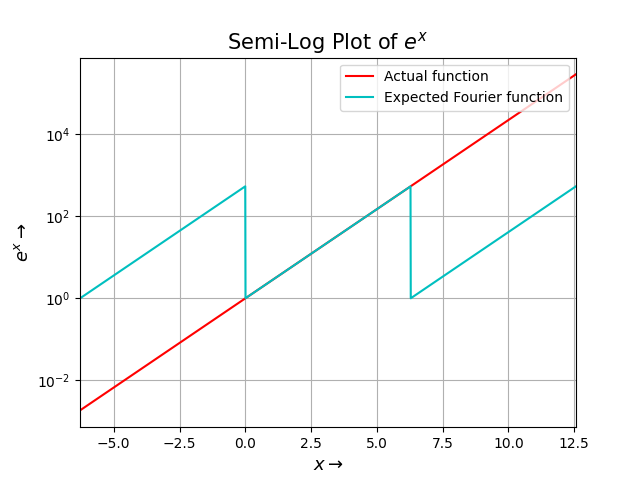
\includegraphics[scale = 0.8]{Figure_1.png}
        \label{fig:sample}
    \end{figure}
    \vspace*{-0.5cm}
\begin{center}
    Since the fourier coefficients are calculated over an interval $[0,2\pi)$, the function generated by fourier coefficients is also periodic with period $2\pi$
\end{center}
\subsubsection{Figure 2: For $\cos(\cos(x))$ function:}
\vspace*{-0.5cm}
    \begin{figure}[H]
        \centering
        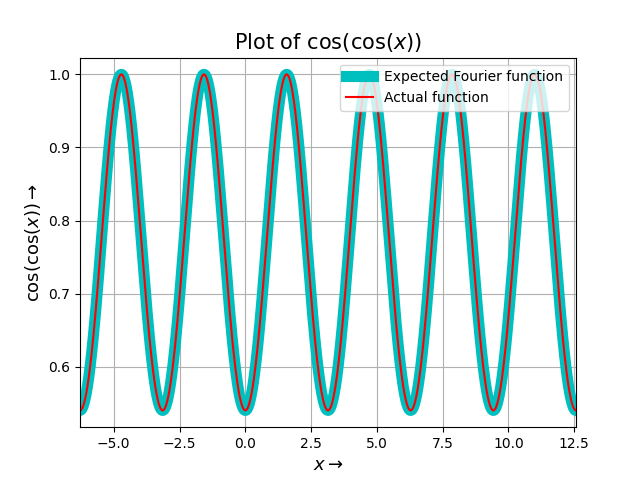
\includegraphics[scale = 0.75]{Figure_2.png}
        \label{fig:sample}
    \end{figure}
\vspace*{-0.5cm}
    \begin{center}
    $\cos(\cos(x))$ is already periodic with period $\pi$. Hence the expected fourier plot is exactly overlapping with the exact function plot.
\end{center}

\subsection{Fourier coefficients obtained by integration}
\subsubsection{Figure 3: Semi-logy plot for the integration coefficients of $e^{x}$:}
\vspace*{-0.5cm}
\begin{figure}[H]
        \centering
        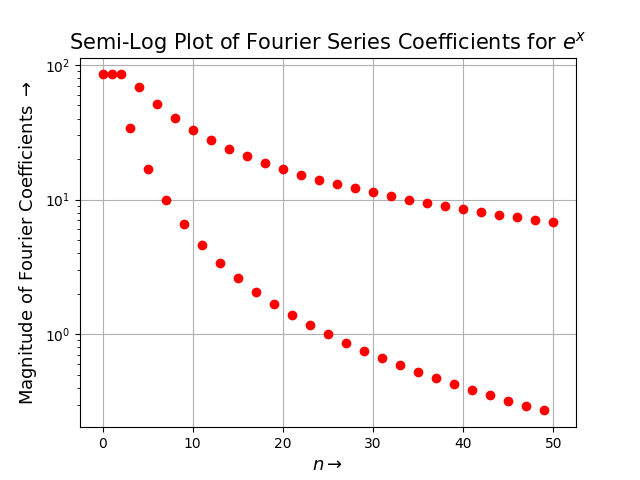
\includegraphics[scale = 0.75]{Figure_3.png}
        \label{fig:sample}
    \end{figure}
\vspace*{-0.5cm}
    \begin{center}
        For function $e^{x}$, the coefficient magnitudes seem to decrease with $n$ in the semilog plot
    \end{center}
\subsubsection{Figure 4: Loglog plot for the integration coefficients of $e^{x}$:}
\vspace*{-0.5cm}
\begin{figure}[H]
    \centering
    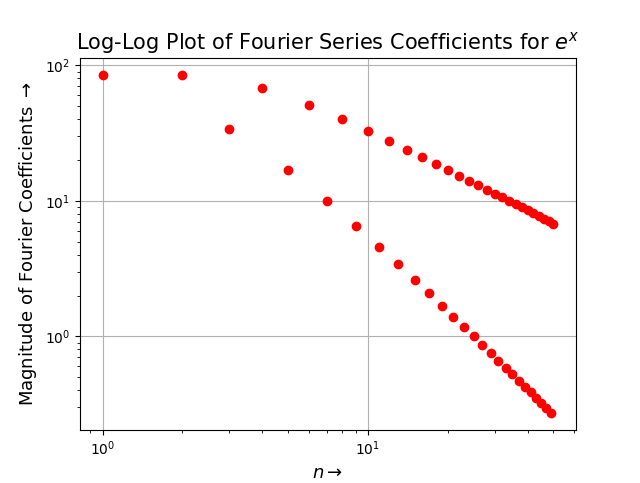
\includegraphics[scale = 0.75]{Figure_4.png}
    \label{fig:sample}
\end{figure}
\vspace*{-0.5cm}
\begin{center}
    For function $e^{x}$, the coefficient magnitudes seem to decrease linearly with $n$ in the loglog plot
\end{center}
\subsubsection{Figure 5: Semi-logy plot for the integration coefficients of $\cos(\cos(x))$:}
\vspace*{-0.5cm}
\begin{figure}[H]
    \centering
    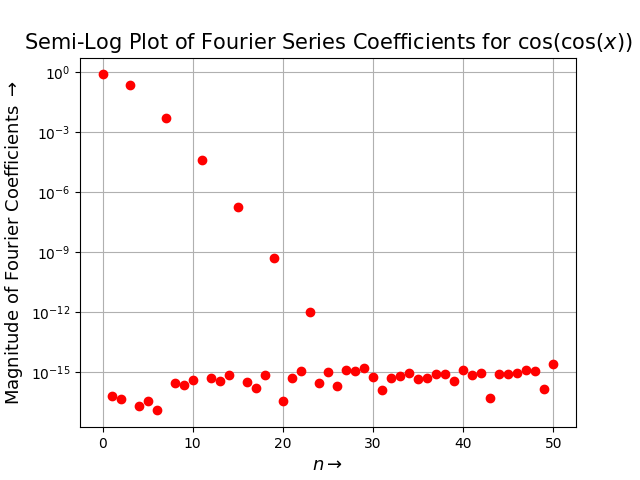
\includegraphics[scale = 0.75]{Figure_5.png}
    \label{fig:sample}
\end{figure}
\vspace*{-0.5cm}
\begin{center}
    For function $\cos(\cos(x))$, the coefficient magnitudes seem to decrease linearly with $n$ in the semilog plot
\end{center}
\subsubsection{Figure 6: Loglog plot for the integration coefficients of $\cos(\cos(x))$:}
\vspace*{-0.5cm}
\begin{figure}[H]
    \centering
    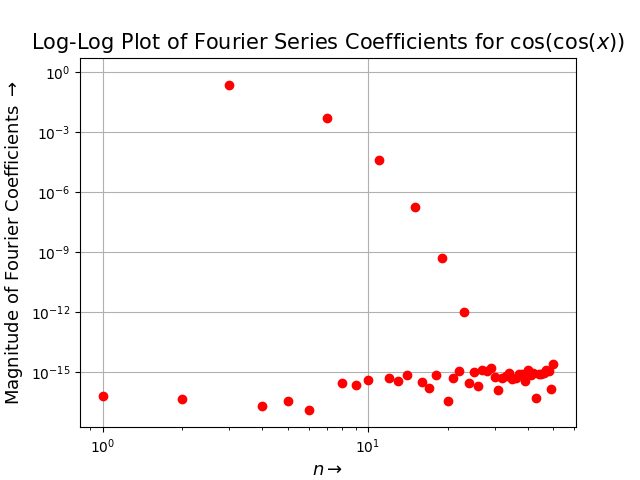
\includegraphics[scale = 0.75]{Figure_6.png}
    \label{fig:sample}
\end{figure}
\vspace*{-0.5cm}
\begin{center}
    For function $\cos(\cos(x))$, the coefficient magnitudes seem to decrease with $n$ in the loglog plot
\end{center}

\subsection{Fourier coefficients obtained by least squares method}
\subsubsection{Figure 7: Semi-logy plot for the least square coefficients of $e^{x}$:}
\vspace*{-0.5cm}
\begin{figure}[H]
        \centering
        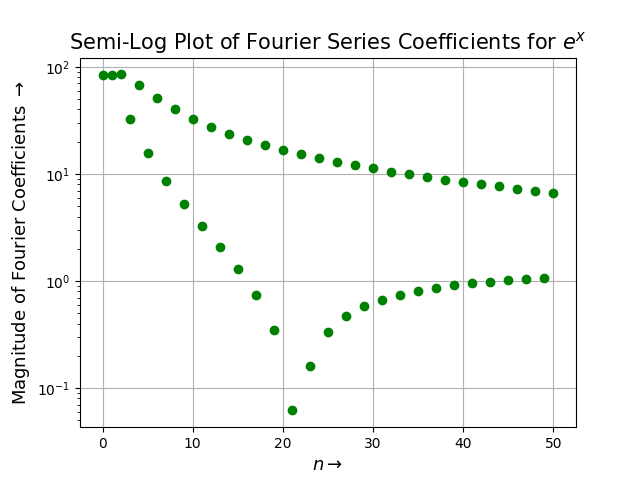
\includegraphics[scale = 0.75]{Figure_7.png}
        \label{fig:sample}
    \end{figure}
\vspace*{-0.5cm}
    \begin{center}
        For function $e^{x}$, the coefficient magnitudes seem to decrease with $n$ in the semilog plot
    \end{center}
\subsubsection{Figure 8: Loglog plot for the least square coefficients of $e^{x}$:}
\vspace*{-0.5cm}
\begin{figure}[H]
    \centering
    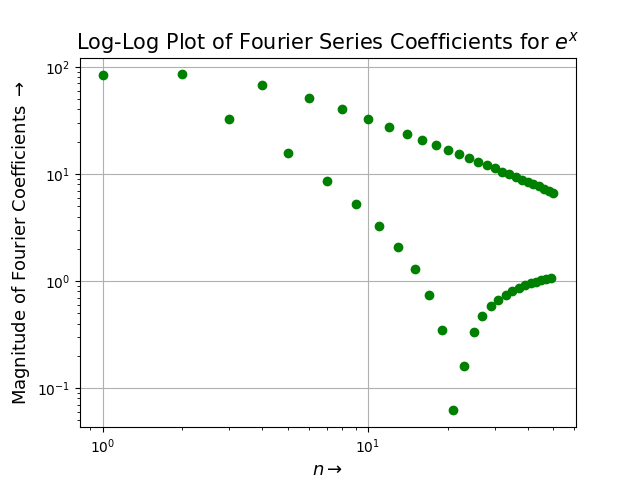
\includegraphics[scale = 0.75]{Figure_8.png}
    \label{fig:sample}
\end{figure}
\vspace*{-0.5cm}
\begin{center}
    For function $e^{x}$, the coefficient magnitudes seem to decrease linearly with $n$ in the loglog plot
\end{center}
\subsubsection{Figure 9: Semi-logy plot for the least square coefficients of $\cos(\cos(x))$:}
\vspace*{-0.5cm}
\begin{figure}[H]
    \centering
    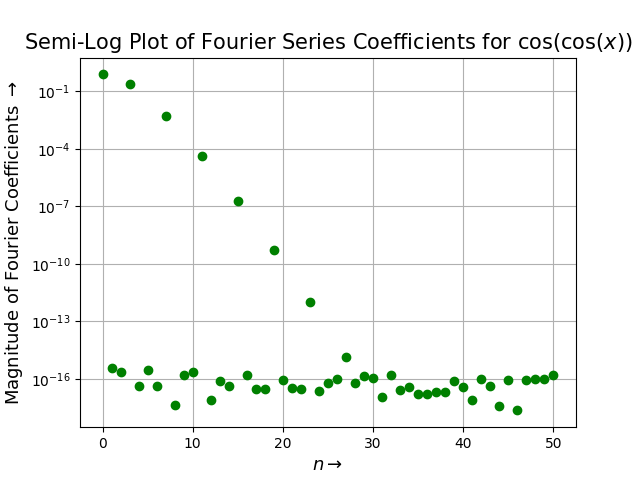
\includegraphics[scale = 0.75]{Figure_9.png}
    \label{fig:sample}
\end{figure}
\vspace*{-0.5cm}
\begin{center}
    For function $\cos(\cos(x))$, the coefficient magnitudes seem to decrease linearly with $n$ in the semilog plot
\end{center}
\subsubsection{Figure 10: Loglog plot for the least square coefficients of $\cos(\cos(x))$:}
\vspace*{-0.5cm}
\begin{figure}[H]
    \centering
    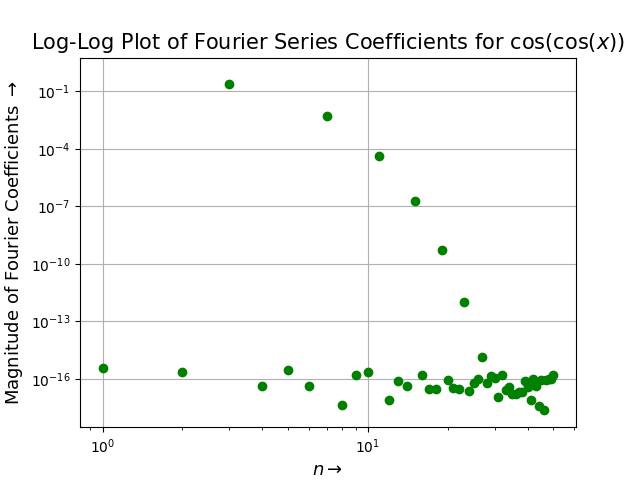
\includegraphics[scale = 0.75]{Figure_10.png}
    \label{fig:sample}
\end{figure}
\vspace*{-0.5cm}
\begin{center}
    For function $\cos(\cos(x))$, the coefficient magnitudes seem to decrease with $n$ in the loglog plot
\end{center}

\subsection{Fourier coefficients obtained by integration vs least squares \\ approximation:}
\subsubsection{Figure 11: Semi-logy plot for the coefficients of $e^{x}$:}
\vspace*{-0.5cm}
\begin{figure}[H]
        \centering
        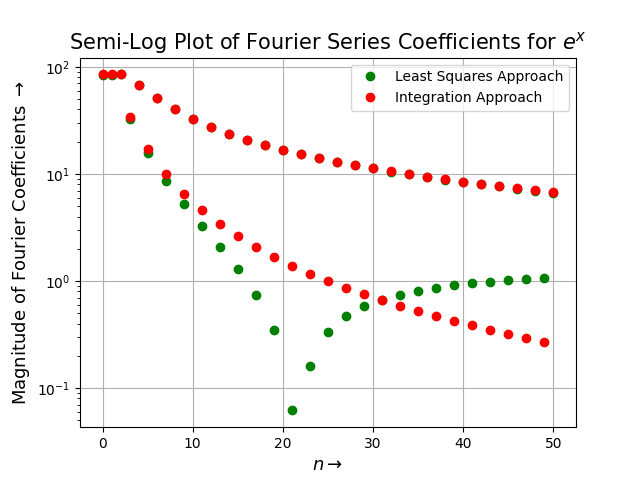
\includegraphics[scale = 0.75]{Figure_11.png}
        \label{fig:sample}
    \end{figure}
\vspace*{-0.5cm}
    \begin{center}
        For function $e^{x}$, the coefficient magnitudes seem to decrease with $n$ in the semilog plot
    \end{center}
\subsubsection{Figure 12: Loglog plot for the coefficients of $e^{x}$:}
\vspace*{-0.5cm}
\begin{figure}[H]
    \centering
    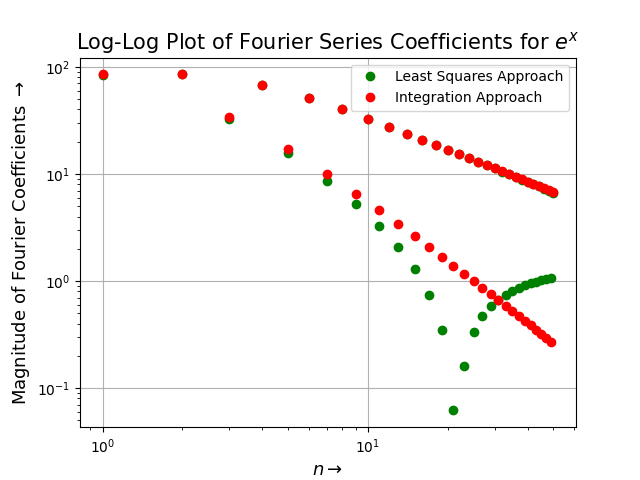
\includegraphics[scale = 0.75]{Figure_12.png}
    \label{fig:sample}
\end{figure}
\vspace*{-0.5cm}
\begin{center}
    For function $e^{x}$, the coefficient magnitudes seem to decrease linearly with $n$ in the loglog plot
\end{center}
\subsubsection{Figure 13: Semi-logy plot for the coefficients of $\cos(\cos(x))$:}
\vspace*{-0.5cm}
\begin{figure}[H]
    \centering
    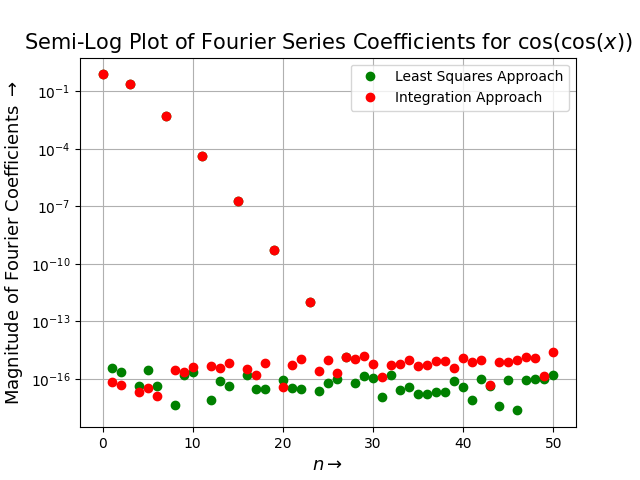
\includegraphics[scale = 0.75]{Figure_13.png}
    \label{fig:sample}
\end{figure}
\vspace*{-0.5cm}
\begin{center}
    For function $\cos(\cos(x))$, the coefficient magnitudes seem to decrease linearly with $n$ in the semilog plot
\end{center}
\subsubsection{Figure 14: Loglog plot for the coefficients of $\cos(\cos(x))$:}
\vspace*{-0.5cm}
\begin{figure}[H]
    \centering
    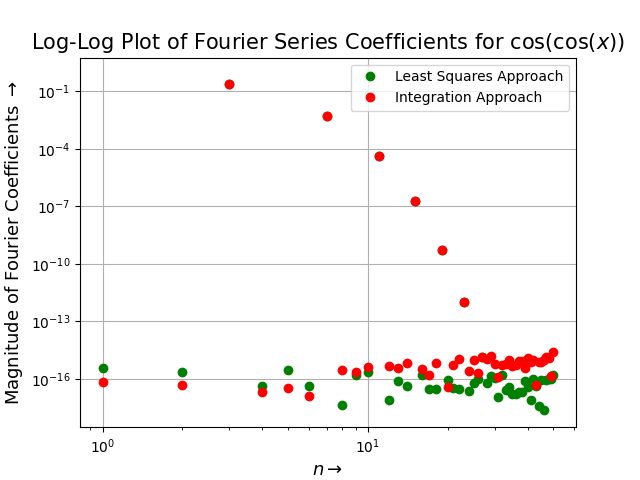
\includegraphics[scale = 0.75]{Figure_14.png}
    \label{fig:sample}
\end{figure}
\vspace*{-0.5cm}
\begin{center}
    For function $\cos(\cos(x))$, the coefficient magnitudes seem to decrease with $n$ in the loglog plot
\end{center}

\subsection{Expected Fourier plot along with Fourier plot obtained using integration coefficients}
\subsubsection{Figure 15: For $e^{x}$ function:}
\vspace*{-0.5cm}
\begin{figure}[H]
        \centering
        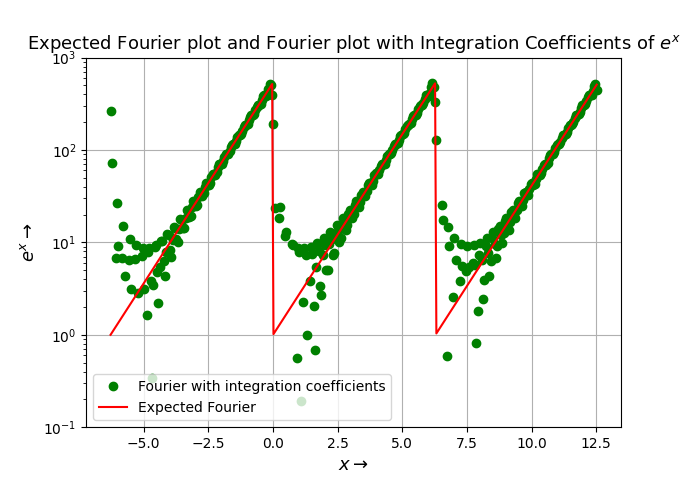
\includegraphics[scale = 0.7]{Figure_15.png}
        \label{fig:sample}
    \end{figure}
\vspace*{-0.5cm}
    \begin{center}
        The function plot generated using fourier coefficients (Integration method) almost match the expected fourier plot, except at the discontinuous points of $e^{x}$ 
    \end{center}
\subsubsection{Figure 16: For $\cos(\cos(x))$ function:}
\vspace*{-0.5cm}
\begin{figure}[H]
    \centering
    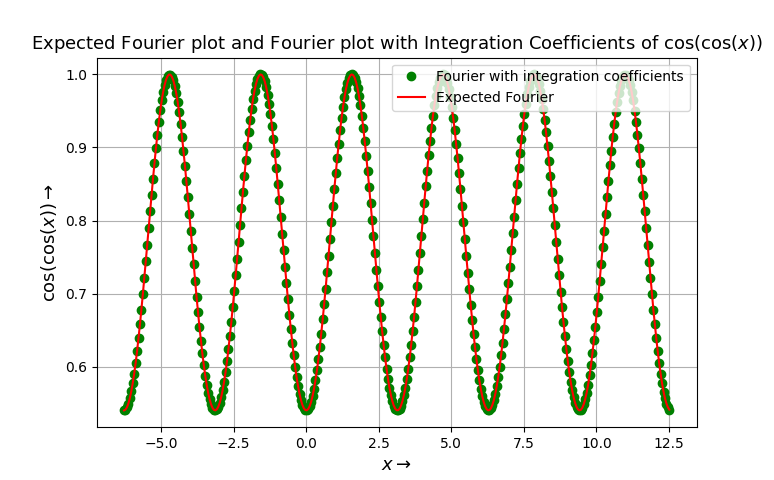
\includegraphics[scale = 0.7]{Figure_16.png}
    \label{fig:sample}
\end{figure}
\vspace*{-0.5cm}
\begin{center}
    The function plot generated using fourier coefficients (Integration method) matches the expected fourier plot almost exactly  
\end{center}

\subsection{Expected Fourier plot along with Fourier plot obtained using least square coefficients}
\subsubsection{Figure 17: For $e^{x}$ function:}
\vspace*{-0.5cm}
\begin{figure}[H]
        \centering
        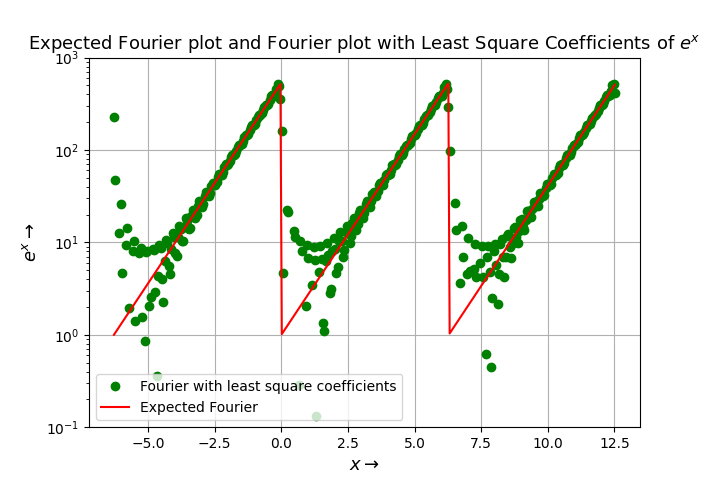
\includegraphics[scale = 0.7]{Figure_17.png}
        \label{fig:sample}
    \end{figure}
\vspace*{-0.5cm}
    \begin{center}
        The function plot generated using fourier coefficients (Least squares method) almost match the expected fourier plot, except at the discontinuous points of $e^{x}$ 
    \end{center}
\subsubsection{Figure 18: For $\cos(\cos(x))$ function:}
\vspace*{-0.5cm}
\begin{figure}[H]
    \centering
    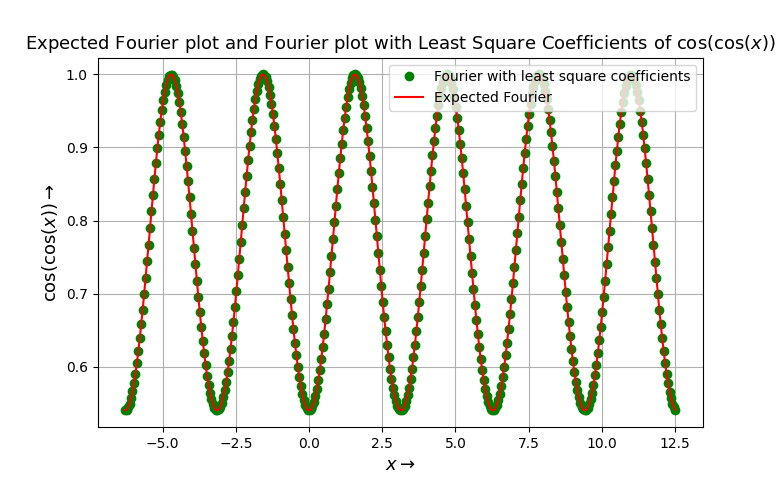
\includegraphics[scale = 0.7]{Figure_18.png}
    \label{fig:sample}
\end{figure}
\vspace*{-0.5cm}
\begin{center}
    The function plot generated using fourier coefficients (Least sqaures method) matches the expected fourier plot almost exactly  
\end{center}

\section{Results and Conclusions}
\subsection{Conclusions for question 3}
\begin{enumerate}[label=\alph*.]
    \item We know that
\begin{equation}
    b_{n} = \int_{0}^{2\pi} \cos(\cos(x))sin(nx)dx
\end{equation}
which translates to
\begin{equation*}
    b_{n} = \int_{0}^{2\pi} \cos(\cos(2\pi-x))sin(n(2\pi-x))dx
\end{equation*}
because of the definite integral identity
    \begin{equation*}
        \int_{a}^{b} f(x)dx = \int_{a}^{b} f(a+b-x)dx
    \end{equation*}
Hence, 
\begin{equation}
    b_{n} = -\int_{0}^{2\pi} \cos(\cos(x))sin(nx)dx
\end{equation}
because $\cos(2\pi-x) = \cos(x)$ and $\sin(n(2\pi-x)) = -\sin(nx)$\\
Adding equations (1) and (2), we get $2b_{n} = 0$. Hence $b_{n} = 0$.
Theoretically $b_{n} = 0$ for all $n$. However because of computer precision the values are not exactly zero but very low (in the order of $10^{-17}$). Hence they decay faster as compared to $a_{n}$ values.
\clearpage
    \item For $e^{x}$:
    \begin{equation*}
        a_{0} = \frac{e^{2\pi}-1}{2\pi}
    \end{equation*}

    \begin{equation*}
        a_{n} = \frac{e^{2\pi}-1}{\pi(n^{2}+1)}
    \end{equation*}

    \begin{equation*}
        b_n = \frac{-n(e^{2\pi}-1)}{\pi(1+n^{2})}
    \end{equation*}

    For $\cos(\cos(x))$, the exact formulae for the coefficients are not known. So we use the Taylor series approximation:

    \begin{equation*}
        \cos(\cos(x)) = 1 - \frac{\cos^{2}x}{2!} + \frac{\cos^{4}x}{4!} - \frac{\cos^{6}x}{6!} + \ldots ,   |\cos(x)|<1
    \end{equation*}
From the above expansion, if we express the $\cos^{2}x$ terms in terms of $\cos2x$, $\cos^{2}2x$ in terms of $\cos4x$ and so on, we see that the fourier coefficients decay exponentially.
Whereas the fourier coefficients of $e^{x}$ decay as $\frac{1}{n^{2}}$. Hence the coefficients of $e^{x}$ do not decay as quickly as the coefficients of $\cos(\cos(x))$.
    \item From part (b) we saw: 
    
    \begin{equation*}
        a_{n} = \frac{e^{2\pi}-1}{\pi(n^{2}+1)}
    \end{equation*}

    \begin{equation*}
        b_n = \frac{-n(e^{2\pi}-1)}{\pi(1+n^{2})}
    \end{equation*}

    Hence for large values of '$n$', we can safely assume that the denominator is approximately $n^{2}$. Hence, we have:

    \begin{equation*}
        \log(|a_{n}|) = \log(\frac{e^{2\pi}-1}{\pi}) - 2\log(n)
    \end{equation*}

    \begin{equation*}
        \log(|b_{n}|) = \log(\frac{e^{2\pi}-1}{\pi}) - \log(n)
    \end{equation*}

That's why we almost have a linear plot in Figure 4, which is the loglog plot of the fourier coefficients of $e^{x}$.

The coefficients of $\cos(\cos(x))$ converge to an exponentially decaying function. That's why we have a linear plot in Figure 5, which is the semilogy plot of the fourier coefficients of $\cos(\cos(x))$.

\subsection{Conclusions for question 6}
The fourier coefficients obtained by the integration and least squares method are different from each other because they have
been calculated using different methods. They will have deviations from one another. However both of them fit the function quite
accurately as seen in Figures 15, 16, 17, 18. The python code snippet used to calculate the deviation is:

\begin{py_code}
    exp_coeff_diff = abs(exp_fourier_coeff - exp_lstsq_coeff)
    print("The largest deviation between the fourier coefficients and least square coefficients of exp(x) is %f" %(np.amax(exp_coeff_diff)))
    
    cos_cos_coeff_diff = abs(cos_cos_fourier_coeff - cos_cos_lstsq_coeff)
    print("The largest deviation between the fourier coefficients and least square coefficients of cos(cos(x)) is ",end = '')
    print(np.amax(cos_cos_coeff_diff))
\end{py_code}
\vspace*{0.4cm}
The results obtained are:
\begin{itemize}
    \item The largest deviation between the fourier coefficients and least square coefficients of $e^{x}$ is 1.332731
    \item The largest deviation between the fourier coefficients and least square coefficients of $\cos(\cos(x))$ is 2.758669e-15
\end{itemize}

\subsection{Conclusions for question 7}
In figures 16 and 18 (Plot of expected fourier for $\cos(\cos(x))$ vs plot obatined from fourier coefficients), there is no much deviation and the green circles almost lie on the expected fourier plot. However we have a lot of deviations from the expected fourier plots in figures 15 and 17 (Plot of expected fourier for $e^{x}$ vs plot obtained from fourier coefficients). Especially the green circles are randomly placed near the discontinuities of $e^{x}$.
This is a result of Gibbs phenomena. It says that the $n$th partial sum of the Fourier series will have large oscillations at the jump discontinuities. As a result of this $e^{x}$ was showing large variations at jumps.

\end{enumerate}

\end{document}